% Chapter 1

\chapter{Introduction} % Write in your own chapter title
\label{Chapter1}
\lhead{Chapter 1. \emph{Introduction}} % Write in your own chapter title to set the page header


\section{Neutron Interferometry}
\subsection{History}
Interferometry has long been a powerful tool for experimental physics. Its various forms have been used in the discovery of many historically significant results such as the Michelson-Morley experiment which showed that the speed of light was independent of inertial reference frames and experimental data in support of Bell's Inequality. \cite{michelson_morley}\cite{bells_inequality}

The key concept of interferometry is the superposition of waveforms upon each other in order to deduce meaningful physical properties from the resultant combination. If one considers two waves of identical frequency than the waves when superimposed will combine constructively when in phase and de-constructively when out of phase. The technique of interferometry can be applied to many different experimental systems, the requirement being that the interferometry medium be described as a wave mathematically. Such systems that have been used in the past include electromagnetic waves, water waves, electrons and neutrons. Although electrons and neutrons classically are described as point particles the development of quantum mechanics allows that all matter is actually described by a waveform and therefore interferometry techniques may be applied to the electron and neutron waveforms. This paper focuses primarily on neutron interferometry. 

The first Neutron Interferometer with slow neutrons was constructed by Maier-Leibnitz and Springer in 1962 and was effectively equivalent to a double slit experiment. However, their interferometer was not effective for measuring physical properties of materials. In 1965 the perfect single-crystal interferometer was theorized by Ulrich Bonse and Michael Hart, however it was not until 1974 that their interferometer was made functional by Helmut Raunch and his student Wolfgang Treimer. Their interferometer used a single perfect crystal in which two horizontal slices were removed from the interior to form a three-blade interferometer.\cite{neutron_history} Using the single-crystal design researchers Colella,Overhauser and Werner to perform the famous COW experiment which measured the phase shift due to the gravitational potential difference between two neutron beams separated by a small displacement in height.\cite{cow} Further experiments made such contributions to experimental physics such as the measurement of the Aharonov-Bohm effect and the the effect of the Earth's rotation on a quantum system.\cite{neutron_history} It was quickly realized that neutron interferometry measurements provide an incredible level of accuracy and isolation in experimental measurements. This is due to the fact that the neutron has essentially zero electric charge and therefore does not feel the Coulomb force. Therefore for the case of slow neutrons there is no need to isolate for stray electric fields. 
\begin{figure}[ht!]
\centering
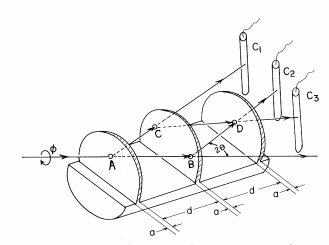
\includegraphics[scale=1.0]{Figures/cow.png}
\caption{An illustration of the interferometer used in the COW experiment.\cite{cow}}
\label{fig:cow}
\end{figure}

\subsection{Application to Quantum Information}
As the neutron interferometry provides a low-noise experimental system it provides an ideal test-bench for testing certain aspects of quantum information theory. Such an example was the use of a five-blade interferometer which allowed the quantum information encoded in the neutron waveform by using additional blades to exploit the symmetry of mechanical vibrations in the interferometer and decouple these modes.\cite{five_blade}. This is an example of encoding the information into a decoherence-free subspace and is a technique that may be applicable in future scalable quantum computation systems. Additionally it has been shown that neutron interferometers can be used for the generation of single neutron entangled states. \cite{neutron_entanglement}   Additionally there is interest in the quantum discord of neutron interferometry systems and there application towards non-classical discord algorithms.\cite{noise_neutron}. It is unlikely that a scalable quantum computer will be realizable with neutrons due to their low interaction with other quantum systems.  
\subsection{Application to Quantum Fundamentals}
Neutron interferometry has played a large role in experimentally gathering information on the fundamental behaviour of quantum systems. Such as the Aharonov-Bohm effect, the effect of gravity,quantum discord and verifying Bell's Inequality. \cite{neutron_history}\cite{cow}\cite{noise_neutron}\cite{bells_inequality}. More recently researchers at the Institute for Quantum Computing are designing an experimental neutron interferometer that is equivalent to a triple-slit experiment in the search for third order interference effects that are theoretically non-existent but if found may be evidence of new quantum theories.\cite{three_slit} 
\subsection{National Institute of Standards and Technology}
The majority of the work presented in this thesis applies directly to the neutron interferometry setup at the National Institute of Standards and Technology in Gaithersburg, MD. The neutrons are produced at the NIST Research Reactor and extracted via a dual-crystal parallel-tracking monochromator with energy of $4-20 meV$. They are fed along wave-guides to the isolated interferometry setup. NIST has three,four and five blade perfect single-crystal interferometry assemblies although we focus on solely the three blade assembly. Neutron detection is provided by $^3He$ detectors or by high resolution position-sensitive detectors.\cite{nist_setup}\cite{nist_powerpoint} 

\begin{figure}[ht!]
\centering
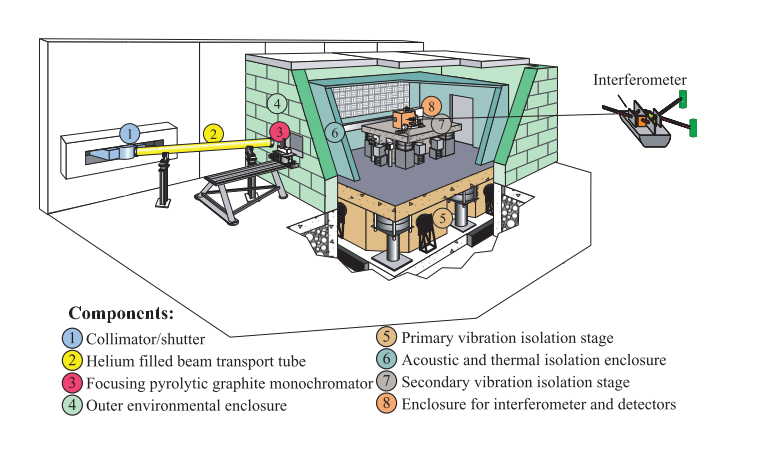
\includegraphics[scale=0.5]{Figures/neutroninterferometer.png}
\caption{Neutron interferometry lab at NIST \cite{dimaThesis}}
\label{fig:neutroninterferometerlab}
\end{figure}
\section{Markov Chain Monte Carlo Methods}
Often in advanced quantum physics the probability distributions of the systems reside in a high dimensional parameter space. It is often desired to find the correct set of parameters to describe a system. However, it is normally impossible to test every single possible real value of the parameter space as the computational time would be astronomical. Markov Chain Monte Carlo methods attempt to solve this problem by using a bunch of "guesses" that will according to a heuristic attempt to reasonably explore the parameter space for the approximate parameters after many iterations.  Markov Chain Monte Carlo Methods have many uses including in Bayesian statistics, physics, biology and linguistics.\cite{mcmc}

The Markov Chain Monte Carlo method can be thought of scattering a large number of particles in a space to be explored. By moving these particles around the space, it is possible to effectively sample the entire space if enough iterations and particles are used. We will use MCMC methods to explore the parameter space of neutron detection probability distributions in order to obtain the optimal set of system parameters. 
\begin{figure}[ht!]
\centering
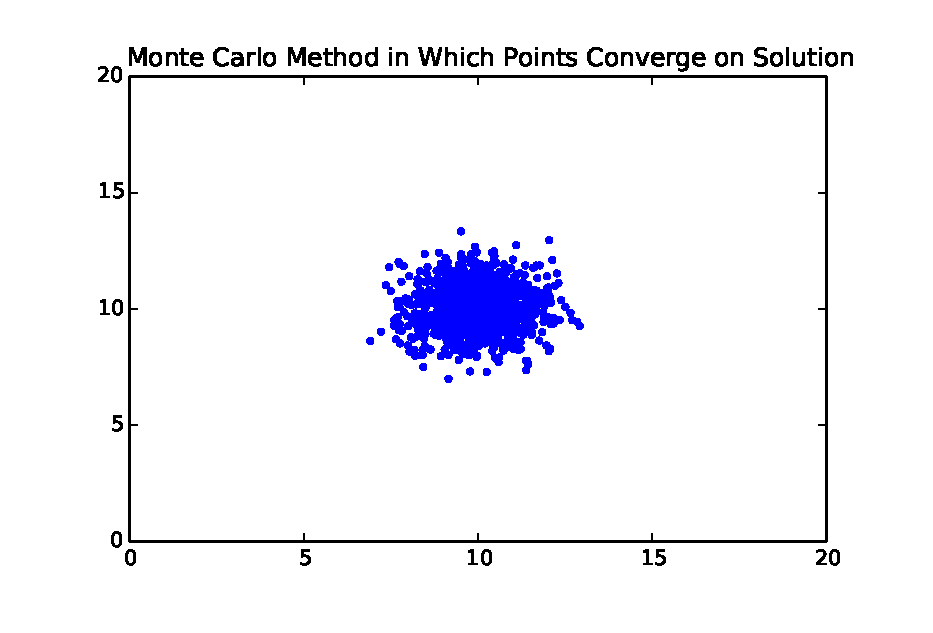
\includegraphics[scale=1.0]{Figures/mcmc.eps}
\caption{Markov Chain Monte Carlo method converging on solution at $(10,10)$}
\label{fig:mcmc}
\end{figure}